\section{Evaluation}
\label{sec:evaluation}

%\begin{enumerate}
%    \item Benchmarks (describe our benchmarks)
%    \item Results (total time, split out SMPT time from our rust code time)
%    \item Analysis of optimizations (how much time they save, petri net sizes, semilinear set sizes)
%    \item Limitations (examples we cannot solve, future work that would help)
%\end{enumerate}


\noindent
\textbf{Experimental Setup.}
All experiments ran on a second generation Lenovo Notebook ThinkPad P16s, with 16 AMD cores and a RAM of 58 GB, with a Linux Ubuntu 24.04.2 operating system.
%
We plan on making all our code, benchmarks raw results publicly available with the final version of this paper.
%
For the underlying Petri Net reachability solver we used SMPT~\cite{AmDa23}, a state-of-the-art reachability solver which supports \textit{unbounded} reachability queries, and which we extended to support our setting (for example, we needed to extend the solver to support proof generation). 
%
We note that other off-the-shelf solvers can be used as well.
%
All our code, benchmarks, and raw experimental results will be made publicly available with the final version of this paper.
 


\subsection{Benchmarks Overview} 
\label{subsec:benchmarks}

\begin{itemize}
	
	\item \todo{update benchmark overview and category names}
	\item \textbf{Core expressions \& multi request workflows}: Benchmarks testing arithmetic, boolean, and simple control expression.
	\item \textbf{Fred (mixed arithmetic)}: Mixed control and arithmetic transformations (Fred series).
	\item \textbf{Stop (circular-increment) series}: Circular increment loops and variants.
	\item \textbf{Concurrency \& locking loops}: Concurrent looping patterns with locking and tricky interactions.
	\item \textbf{Non-deterministic choice \& randomness}: Random choice and non-deterministic branching benchmarks.
	\item \textbf{Networking \& system protocols}: Networking protocols and system-level monitoring.
	\item \textbf{JSON state-machine examples}: Example JSON-encoded state machine workflows.
\end{itemize}



The benchmarks differ in their complexity and in the various features pertaining to them --- branching, loops, randomness, multiple requests, etc. 
%

\subsection{Runtime Results}
We ran our tool on all 47 benchmarks, out of which 27 are serializable programs, and the remaining 20 are non serializable benchmarks. 
For each benchmark, we measured the time for deciding the reachability query, indicating serializability, as well as the overall time, including validation of the invariant proof (if serializable) or the validation of the counterexample (if not serializable). These experiments ran in parallel, with $16$ cores, an a \texttt{TIMEOUT} threshold of 500 seconds and with all four optimizations. As can be seen by our results (summarized in Table~\ref{tab:benchmarks-all}), withing this time limit, our tool full solved 26/27 serializable benchmarks 
and 19/20 no serializable benchmarks. 
%
The \textit{average} total runtime was $52{,}857.55$ ms across all benchmarks, and $25{,}530.69$ ms ($42{,}980.47$ ms) when focusing on solely serializable (non-serializable) benchmarks.
%
The \textit{median} total runtime was $2{,}080$ ms across all benchmarks, and $2{,}238.50$ ms ($830$ ms) when focusing on solely serializable (non-serializable) benchmarks.
%
We also note that when analyzing the benchmarks based on their serializability, there is a clear difference in their average runtime --- while in the serializable benchmarks the validation of the certificate takes significantly longer than generating the certificate (i.e., the proof) --- in the non serializable benchmarks this trend is reversed, with the total average time being dominated by the generation of the counterexample. This of course is not surprising, as counterexample generation can be done in polynomial time by emulating our \todo{PN? System} system and checking that the final counterexample can be attained.
%
We report the full results in Table~\ref{tab:stats-summary}, and elaborate on the per-benchmark results in Table~\ref{tab:benchmarks-all}.





\begin{table}[H]
	\centering
	% Load the tabular from the external file:
	\begin{table}[H]
	\centering
	\begin{tabular}{lrrrrrr}
		\toprule
		& \multicolumn{3}{c}{Average time (ms)} & \multicolumn{3}{c}{Median time (ms)} \\
		\cmidrule(lr){2-4} \cmidrule(lr){5-7}
		Category
		& \shortstack{certificate\\generation}
		& \shortstack{certificate\\validation}
		& total
		& \shortstack{certificate\\generation}
		& \shortstack{certificate\\validation}
		& total \\
		\midrule
		Serializable      &   2273 &  23257 &  25531 &  1178 &  1300 &  2238 \\
		Not serializable  &  42076 &    905 &  42980 &   773 &    78 &   830 \\
		All               &  39613 &  13244 &  52858 &   797 &   151 &  2080 \\
		\bottomrule
	\end{tabular}
\end{table}
\caption{Average and median certificate generation, certificate validation, and total running times for serializable, non‐serializable, and all benchmarks. These values are rounded to the nearest integer, to reduce clutter.}
\label{tab:stats-summary}
\end{table}





%=== Overall ===
%Certificate running time:
%Average = 39613.23
%Median  = 797.00
%
%Certificate validation time:
%Average = 13244.32
%Median  = 151.00
%
%Total running time:
%Average = 52857.55
%Median  = 2080.00
%
%=== Serializable Only ===
%Certificate running time:
%Average = 2273.38
%Median  = 1178.00
%
%Certificate validation time:
%Average = 23257.31
%Median  = 1299.50
%
%Total running time:
%Average = 25530.69
%Median  = 2238.50
%
%=== Non-Serializable Only ===
%Certificate running time:
%Average = 42075.84
%Median  = 773.00
%
%Certificate validation time:
%Average = 904.63
%Median  = 78.00
%
%Total running time:
%Average = 42980.47
%Median  = 830.00
%
%=== Percentiles (Overall) ===
%Certificate running time percentiles:
%25th percentile = 553.50
%50th percentile = 797.00
%100th percentile = 502810.00
%
%Certificate validation time percentiles:
%25th percentile = 66.50
%50th percentile = 151.00
%100th percentile = 282370.00
%
%Total running time percentiles:
%25th percentile = 615.00
%50th percentile = 2080.00
%100th percentile = 503336.00
%
%=== Percentiles (Serializable) ===
%Certificate running time percentiles:
%25th percentile = 312.00
%50th percentile = 1178.00
%100th percentile = 9858.00
%
%Certificate validation time percentiles:
%25th percentile = 115.75
%50th percentile = 1299.50
%100th percentile = 282370.00
%
%Total running time percentiles:
%25th percentile = 456.50
%50th percentile = 2238.50
%100th percentile = 292228.00
%
%=== Percentiles (Non-Serializable) ===
%Certificate running time percentiles:
%25th percentile = 628.50
%50th percentile = 773.00
%100th percentile = 356195.00
%
%Certificate validation time percentiles:
%25th percentile = 50.00
%50th percentile = 78.00
%100th percentile = 15227.00
%
%Total running time percentiles:
%25th percentile = 707.00
%50th percentile = 830.00
%100th percentile = 356299.00





\begin{table}[htbp]
	\centering
	% Load the tabular from the external file:
	\begin{table}[H]
	\centering
	\small
	% increase horizontal padding between columns
	\setlength{\tabcolsep}{5pt}
	\renewcommand{\arraystretch}{0.9}
	\begin{tabular*}{\textwidth}{@{\extracolsep{\fill}}%
			p{1.5cm}   % Category
			p{1.0cm} % Benchmark
			c        % Serializable
			c c c c c c % Features
			r r       % Cert, Total
		}
		\toprule
		\multicolumn{2}{c}{\textbf{Benchmark}}
		& \textbf{Serializable}
		& \multicolumn{6}{c}{\textbf{Features}}
		& \multicolumn{2}{c}{\textbf{Runtime (ms)}} \\
		\cmidrule(lr){1-2} \cmidrule(lr){3-3} \cmidrule(lr){4-9} \cmidrule(lr){10-11}
		&
		&
		& If & While & \texttt{?} & Arith & Yield & Multi-req
		& Cert. & Total \\
		\midrule
		\multirow{7}{=}{Core expressions} & \texttt{a1.ser} & \greencmark &  & \cmark &  &  &       &   & 2 & 47 \\
		 & \texttt{a2.ser} & \xmark &  &        &  &  & \cmark &   & 280 & 296 \\
		 & \texttt{a3.ser} & \greencmark &  &        &  &  &       &   & 1 & 32 \\
		 & \texttt{a4.ser} & \greencmark &  &        &  &  & \cmark & \cmark & 637 & 1071 \\
		 & \texttt{a5.ser} & \greencmark &  & \cmark &  &  & \cmark & \cmark & 3234 & 13624 \\
		 & \texttt{a6.ser} & \xmark &  &        &  &  & \cmark & \cmark & 757 & 775 \\
		 & \texttt{a7.ser} & \greencmark & \cmark & \cmark &  &  & \cmark &   & 4 & 33 \\
		\midrule
		\multirow{4}{=}{State machines} & \texttt{b1.json} & \greencmark & \cmark &        &  &  & \cmark & \cmark & 683 & 968 \\
		 & \texttt{b2.json} & \greencmark & \cmark &        &  &  & \cmark & \cmark & 2063 & 7802 \\
		 & \texttt{b3.json} & \greencmark & \cmark &        &  &  & \cmark & \cmark & 730 & 2080 \\
		 & \texttt{b4.json} & \greencmark & \cmark &        &  &  & \cmark & \cmark & 660 & 1909 \\
		\midrule
		\multirow{8}{=}{Fred (mixed arithmetic)} & \texttt{c1.ser} & \xmark &  & \cmark &  & \cmark & \cmark & \cmark & 356195 & 356299 \\
		 & \texttt{c2.ser} & \greencmark &  & \cmark &  & \cmark & \cmark & \cmark & 9858 & 292228 \\
		 & \texttt{c3.ser} & \greencmark &  & \cmark &  & \cmark & \cmark & \cmark & 1886 & 2397 \\
		 & \texttt{c4.ser} & \greencmark &  & \cmark &  & \cmark & \cmark & \cmark & 4336 & 7193 \\
		 & \texttt{c5.ser} & \xmark &  & \cmark &  & \cmark & \cmark & \cmark & 43694 & 43735 \\
		 & \texttt{c6.ser} & \xmark &  & \cmark &  & \cmark & \cmark & \cmark & 629 & 698 \\
		 & \texttt{c7.ser} & \xmark &  & \cmark &  & \cmark & \cmark & \cmark & 797 & 875 \\
		 & \texttt{c8.ser} & \greencmark &  & \cmark &  & \cmark & \cmark & \cmark & 4357 & 8931 \\
		\midrule
		\multirow{5}{=}{Circular increment} & \texttt{d1.ser} & \greencmark & \cmark & \cmark & \cmark &  & \cmark &   & 2391 & 5373 \\
		 & \texttt{d2.ser} & \xmark & \cmark &        & \cmark &  &   \cmark &   & 628 & 731 \\
		 & \texttt{d3.ser} & \greencmark & \cmark & \cmark & \cmark &  &  \cmark &   & 2642 & 10266 \\
		 & \texttt{d4.ser} & \greencmark & \cmark & \cmark & \cmark &  &     \cmark &   & 5604 & 22249 \\
		 & \texttt{d5.ser} & \xmark & \cmark &        &  &  & \cmark &   & 495 & 554 \\
		\midrule
		\multirow{7}{=}{Concurrency \& locking loops} & \texttt{e1.ser} & \greencmark &  & \cmark &  &  & \cmark &   & 351 & 502 \\
		 & \texttt{e2.ser} & \xmark & \cmark & \cmark &  & \cmark & \cmark & \cmark & \texttt{TIMEOUT} & \texttt{TIMEOUT} \\
		 & \texttt{e3.ser} & \xmark & \cmark & \cmark &  & \cmark &   \cmark & \cmark & 24899 & 25039 \\
		 & \texttt{e4.ser} & \xmark & \cmark & \cmark &  &  \cmark &   \cmark & \cmark & 273062 & 273351 \\
		 & \texttt{e5.ser} & \greencmark & \cmark & \cmark & \cmark &  & \cmark &   & 2 & 55 \\
		 & \texttt{e6.ser} & \greencmark & \cmark & \cmark & \cmark &  & \cmark &   & 10 & 114 \\
		 & \texttt{e7.ser} & \greencmark &  & \cmark &  &  &   \cmark &   & 299 & 444 \\
		\midrule
		\multirow{9}{=}{Non-deterministic \& randomness} & \texttt{f1.ser} & \greencmark & \cmark &    \cmark    & \cmark &  & \cmark &   & 388 & 494 \\
		 & \texttt{f2.ser} & \xmark & \cmark &   \cmark     & \cmark &  & \cmark &   & 612 & 676 \\
		 & \texttt{f3.ser} & \xmark &  &        &  & \cmark &   \cmark & \cmark & 653 & 716 \\
		 & \texttt{f4.ser} & \greencmark &  &     \cmark   &  & \cmark & \cmark & \cmark & 1626 & 9515 \\
		 & \texttt{f5.ser} & \greencmark & \cmark &        & \cmark &  &       &   & 7401 & 11301 \\
		 & \texttt{f6.ser} & \xmark & \cmark &        & \cmark &  & \cmark &   & 646 & 830 \\
		 & \texttt{f7.ser} & \xmark & \cmark &        & \cmark &  &  \cmark &   & 400 & 427 \\
		 & \texttt{f8.ser} & \xmark & \cmark &        & \cmark &  &   \cmark &   & 773 & 802 \\
		 & \texttt{f9.ser} & \greencmark & \cmark &        & \cmark &  &  \cmark &   & 10 & 94 \\
		\midrule
		\multirow{7}{=}{Networking \& system protocols} & \texttt{g1.ser} & \xmark & \cmark & \cmark &  & \cmark & \cmark & \cmark & 59312 & 74539 \\
		 & \texttt{g2.ser} & \greencmark & \cmark & \cmark &  & \cmark & \cmark & \cmark & \texttt{TIMEOUT} & \texttt{TIMEOUT} \\
		 & \texttt{g3.ser} & \xmark & \cmark & \cmark & \cmark & \cmark & \cmark & \cmark & 20557 & 20954 \\
		 & \texttt{g4.ser} & \xmark & \cmark & \cmark & \cmark & \cmark & \cmark & \cmark & 6859 & 7047 \\
		 & \texttt{g5.ser} & \greencmark & \cmark & \cmark & \cmark & \cmark &   \cmark & \cmark & 3047 & 12324 \\
		 & \texttt{g6.ser} & \xmark & \cmark &        & \cmark & \cmark & \cmark &   & 8193 & 8285 \\
		 & \texttt{g7.ser} & \greencmark & \cmark &        & \cmark & \cmark &       &   & 6886 & 252752 \\
		\midrule
\bottomrule
	\end{tabular*}
\end{table}

	\caption{Overview of benchmarks with combined categories and updated serializability markings. All optimizations were used, as well as a timeout value of 500 seconds.}
\label{tab:benchmarks-all}
\end{table}


\subsection{Optimization Analysis}

For our next batch of experiments, we compared the various combinations of our four optimizations, and analyzed their effect on the overall runtime and space resources.
%
All experiments were run with a \texttt{TIMEOUT} value of $150$ seconds.

\subsubsection{Runtime Optimization}

We ran all benchmarks with each of the following six optimization combinations: 
(i) without any optimization (marked [\texttt{\textbf{\text{-}\text{-}\text{-}\text{-}}}] in Fig.~\ref{fig:timeout_cumulative_solved_log}); (ii) with bidrectional pruning (marked [\texttt{\textbf{\text{B}\text{-}\text{-}\text{-}}}]); (iii) with redundant constraint elimination (marked [\texttt{\textbf{\text{-}\text{R}\text{-}\text{-}}}]); (iv) with generation of fewer constraints (marked [\texttt{\textbf{\text{-}\text{-}\text{G}\text{-}}}]);
(v) with strategic Kleene elimination(marked [\texttt{\textbf{\text{-}\text{-}\text{-}\text{S}}}]);
and finally, with (vi) all optimizations altogether (marked [\texttt{\textbf{\text{B}\text{R}\text{G}\text{S}}}]).
%
The results of the aggregated overall runtimes are presented in Fig.~\ref{fig:timeout_cumulative_solved_log}, and show that over $19\%$ more benchmarks are solved when using all optimizations, compared to running without any optimizations.
%
Not surprisingly, the best configuration is the one with all optimizations on. 
%
We also note that the best single-optimization configurations with regard to runtime are [\texttt{\textbf{\text{-}\text{-}\text{G}\text{-}}}] and [\texttt{\textbf{\text{-}\text{B}\text{-}\text{-}}}], solving over $74\%$ and $72\%$ of the benchmarks respectively. 
%
We also note that the two remaining optimizations, [\texttt{\textbf{\text{R}\text{-}\text{-}\text{-}}}] and [\texttt{\textbf{\text{-}\text{-}\text{-}\text{S}}}], performed slightly worse (although not by much) than without the optimizations when counting overall timeouts.
%
However, when comparing the combinations it seems that there an instances in which each of these optimizations \textit{strictly} improves runtime.
%
For example, there are instances such as \texttt{a3.ser} and \texttt{a7.ser}, in which the use of the redundant constraint optimization (  [\texttt{\textbf{\text{R}\text{-}\text{-}\text{-}}}])
affords a speedup of between $72.2\%-85.2\%$ over the same benchmarks without this optimization.



\begin{center}
	\begin{minipage}[htbp]{0.48\textwidth}
		\centering
		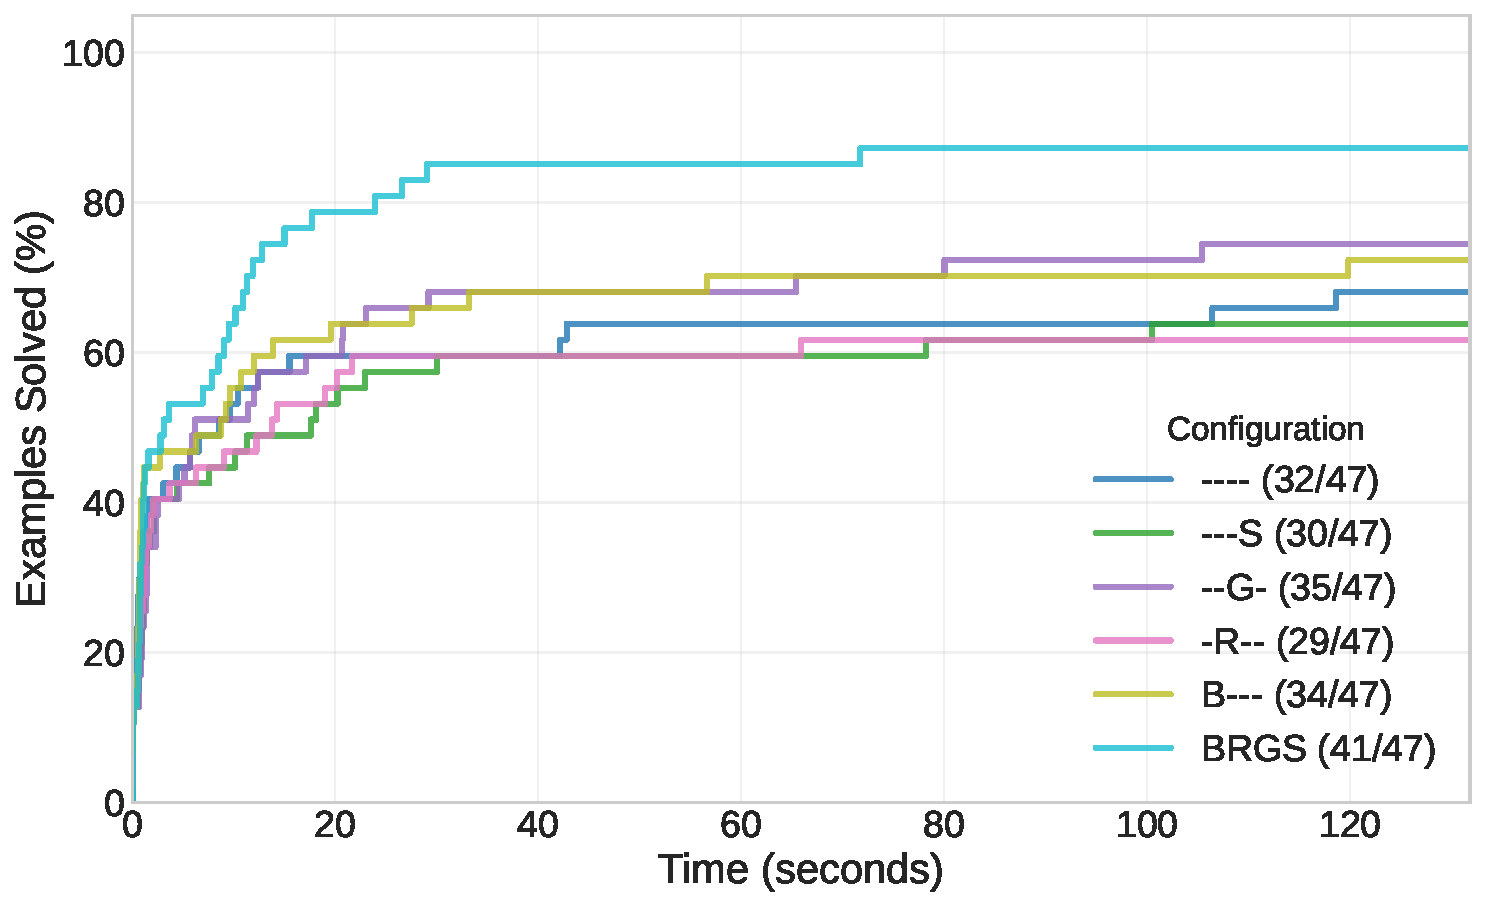
\includegraphics[width=\linewidth]{figures/cactus_plot.pdf}
		\captionof{figure}{Cumulative  solved instances over time.}
		\label{fig:timeout_cumulative_solved_log}
	\end{minipage}\hfill
	\begin{minipage}[htbp]{0.48\textwidth}
		\centering
		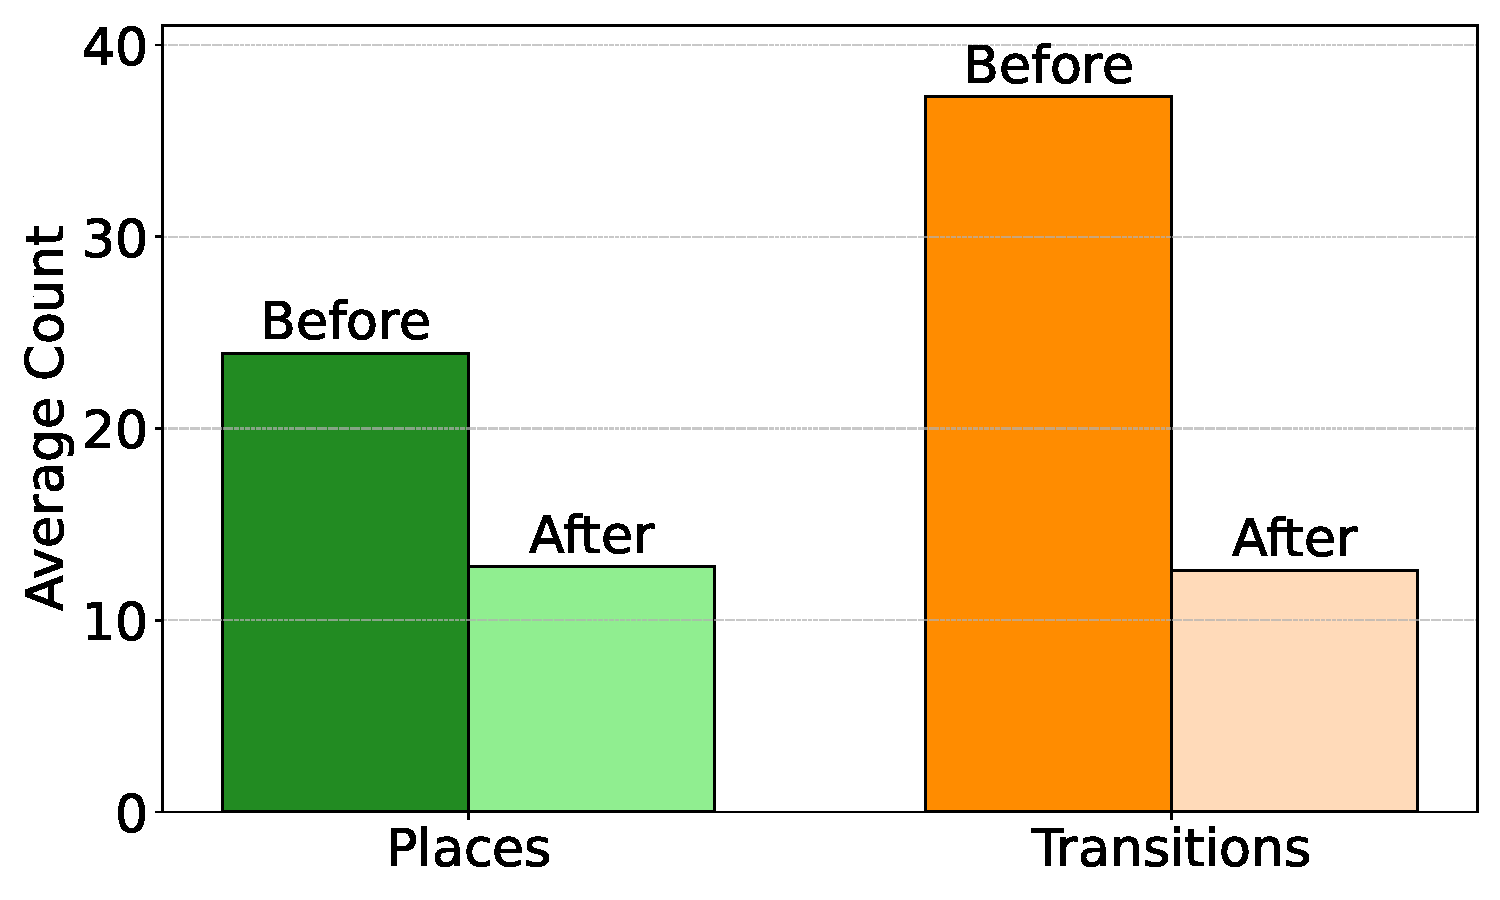
\includegraphics[width=\linewidth]{figures/petri_size_reduction_plot.pdf}
		\captionof{figure}{Reduction of Petri nets size via  pruning.}
			%(timeout 150 seconds)
			%.}
		\label{fig:petri_size_reduction}
	\end{minipage}
\end{center}



\subsubsection{Space Optimization}

In addition to time complexity, out optimizations also allow reducing the space complexity of the two main components pertaining to our approach --- the Petri Net size and the semilinear set size.

\paragraph{Petri Net size reduction.}

With all optimizations enabled, we evaluated the impact of our bidirectional pruning by comparing, across all benchmarks, the average number of places and transitions before and after pruning. On average, pruning cut the number of places \textit{by roughly half} --- dropping from $23.91$ places before pruning to $12.79$ places after. It was even more effective on transitions, \textit{eliminating about two-thirds} of them: from $37.3$ transitions on average before pruning down to $12.61$ after. Note that the pre-pruning averages were computed over $47$ nets (one per benchmark), whereas the post-pruning averages span $224$ nets, since each pre-pruning net produces one pruned net for each disjunct in our reachability query. These results are summarized in Fig.~\ref{fig:petri_size_reduction}.

%When running our tool with all optimizations on, we analyzed the effect of our bidirectional pruning, This was done be counting the average number of places and transitions before and after pruning, on all benchmarks.
%%
%The pruning resulted in a reduction of about half the number of original places --- from $23.91$ places on average \textit{before} pruning to $12.79$ places on average \textit{after} pruning.
%%
%The bidirectional was even more effective in reducing the transitions, as demonstrated by a removing about two thirds of the transitions --- resulting in pruned Petri Nets with $37.30$ transitions on average \textit{before} pruning to $12.61$ transitions on average \textit{after} pruning.
%%
%We note that the averaging for the pre-pruning step was done on $47$ nets, once per each benchmark, while the averaging for the post-pruning step was done on $224$ nets, as each pre-pruning net can give rise to multiple post-pruning nets, one per each disjunct in our reachability query.
%%
%These results are presented in Fig.~\ref{fig:petri_size_reduction}.


%Number of values for 'Before' bars:          47
%Number of values for 'After' bars:           224
%Average number of places before pruning:     23.91
%Average number of places after pruning:      12.79
%Average number of transitions before pruning: 37.30
%Average number of transitions after pruning:  12.61






\paragraph{Semilinear set size reduction.}

Finally, our last batch of experiment analyzed the size reduction in the semilinear set.
%
Towards this end, we ran all our benchmarks with all optimizations, to serve as a baseline. 
%
Then, we analyzed the effect of the three semilinear-related optimizations, i.e., all but the bidirectional pruning which effects the Petri Net size. for each of these three optimizations, we ran the benchmarks with all optimizations \textit{except} the one checked.
%
Table~\ref{tab:semilinear-size-reduction} include a summary of the results, when comparing the semilinear set size.
%
Specifically, we compare both the mean and the average (i) number of components; and (ii) period vectors per each component.
%
As can be seen, the redundant constraint elimination and the generate-less-constraints optimizations had a highly significant effect on the mean and maximal number of components, with the latter being especially effective in reducing the maximal number of components to be $931$ times more compact, and the average number of components to be $223$ more compact, when compared to the baseline.
%
In fact, for both these optimizations are even more effective as, in order to conduct a fair comparison, we analyzed only benchmarks that terminated in all combinations.
%
This, we do not include cases in which these two optimizations rendered the original semilinear set intractable, due to having over $2^30$ components (!), hence timing-out and being excluded from the analysis.
%
This occurs especially in our state-machine serializable benchmarks which have loops in their network systems --- and hence even simple programs of this category cannot be analyzed with respect to serializability.

\todo{understand why this is related to loops in the NS}


\begin{table}[htbp]
	\centering
	% Load the tabular from the external file:
	\begin{table}[H]
	\centering
	\begin{tabular}{l c c c c}
		\toprule
		& \multicolumn{2}{c}{number of components} & \multicolumn{2}{c}{periods per component} \\
		\cmidrule(lr){2-3} \cmidrule(lr){4-5}
		& average & max & average & max \\
		\midrule
	all optimizations (baseline) & 2.91 & 22 & 1.33 & 4 \\
	without remove-redundant & 8.79 & 194 & \textbf{1.64} & 11 \\
	without generate-less & \textbf{651.41} & \textbf{20{,}484} & 1.28 & \textbf{15} \\
	without smart-kleene-order & 2.91 & 22 & 1.35 & 4 \\
  \bottomrule
	\end{tabular}
\end{table}

	\caption{Comparison of experiment runs with a 150-second timeout.}
	\label{tab:semilinear-size-reduction}
\end{table}

\todo{Limitations?}
Examples we cannot solve, future work that would help

%\newpage



